%!TEX root = report.tex
\newpage
\section{Experimental Setup}

\subsection{Overview}

The experimental setup includes 4 cameras for providing ground truth, a speaker and an acoustic head fixed to the robot for recording the room impulse response. A snapshot of this setup at one given position is shown in Figure \ref{fig:overview}.

The steps of one iteration of measures are:
\begin{itemize}
    \item Get images from cameras and perform visual localization.
    \item Read current encoder state.
    \item Record the response to a sine sweep for room impulse response calculation. 
    \item Move the robot to the next position.
\end{itemize}

The above steps are repeated for as many positions as necessary. This procedure is implemented in a program which guides the user through the necessary steps and saves the recorded data in a structured way. 

The instructions for the preparation, setup and operating of the experimental framework can be found online \cite{Instructions}.
\begin{figure}[H]
    \centering
    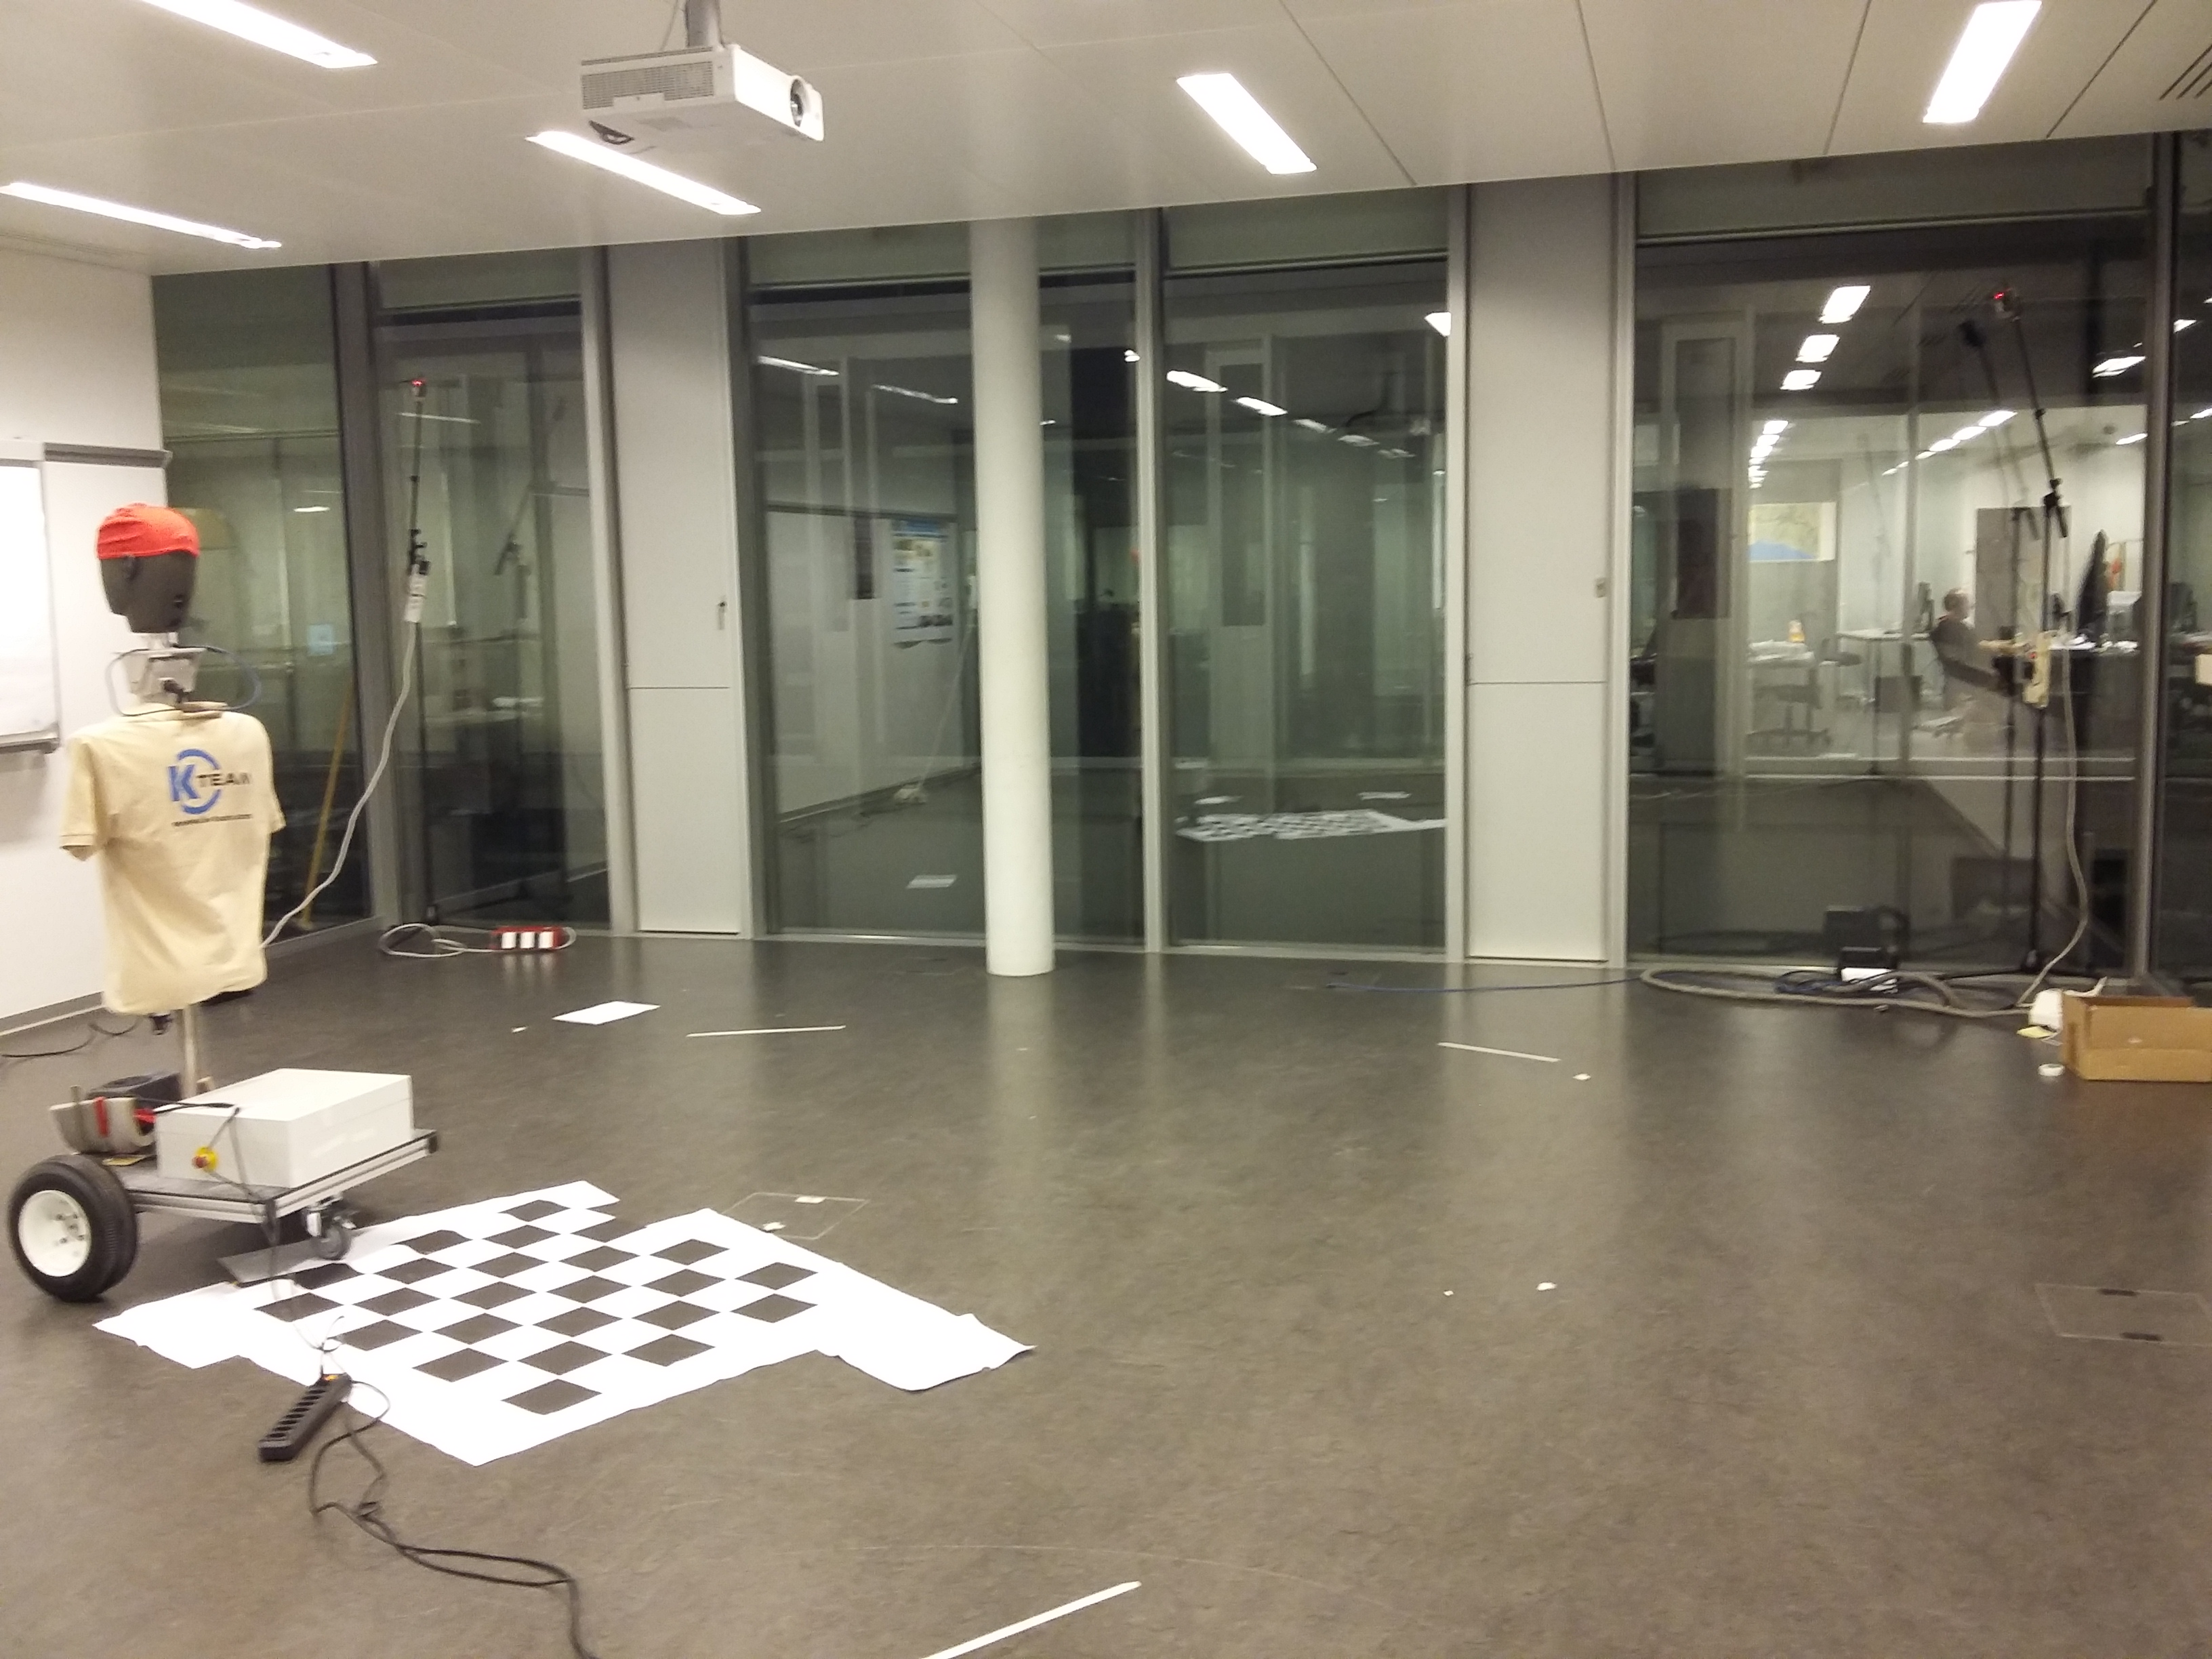
\includegraphics[width=0.6\linewidth]{files/Overview.jpg}
    \caption{Experimental setup with cameras, robot, speaker and checkerboard.}
    \label{fig:overview}
\end{figure}
\subsection{Camera Setup}

\paragraph{Hardware} The camera used is a Raspi-Camera module powered by a \textit{Raspberry Pi 2 Model B}.
The Operating System loaded on the Raspberry Pi is the common Raspian WHEEZY system with some customizations and two custom scripts that are run at startup. 

The camera has the following key parameters \cite{RaspiDoc}
\begin{itemize}
    \item Pixel Count: 2592 $\times$ 1944 (chosen resolution: 1280 $\times$ 720)
    \item Pixel size 1.4 x 1.4 $\mu m$
    \item Focal width and length: $f=3.6mm$
\end{itemize}

\begin{figure}
    \centering
    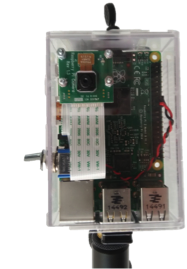
\includegraphics[width=0.25\linewidth]{files/RaspiCam.png}
    \caption{Raspberry Pi with camera module and button used for visual localization.}
    \label{fig:camera}
\end{figure}


\paragraph{Webcam setup} In order to connect to the local network on startup, a few lines of code need to be added in the Rasperry Pi's \texttt{/etc/network/interfaces} 

\begin{center}
\begin{minipage}{0.9\linewidth}
    \begin{lstinputlisting}[caption=\texttt{/etc/network/interfaces}., label=interfaces, frame=none]
        {files/interfaces}
\end{lstinputlisting}
\end{minipage}
\end{center}

The camera module comes with its own library for taking single images ($raspistill$) or videos ($raspivid$).
The following lines of code are added to the file \texttt{$\sim$/start\_camera.sh} in order to take pictures at regular intervals and store them on a local server. 
\begin{center}
\begin{minipage}{0.9\linewidth}
\begin{lstinputlisting}[caption=\texttt{$\sim$/start\_camera.sh}., label=startcamera, frame=none]
    {files/start_camera}
\end{lstinputlisting}
\end{minipage}
\end{center}

Line 5 of Code~\ref{startcamera} captures images of resolution $w\times h = 1280 \times 720$ with ``quality'' $q=10\%$ -- a measure of the image compression. 
The images are captured at a time interval $tl = \u{100}{ms}$ until the time $t = \u{2147483647}{ms} = \u{24}{d}\,\u{19}{h}$ is reached, which is the maximum value for a 32-bit signed integer.
Other parameters like the exposure, set to backlight, and the metering mode can also be set. 

\begin{figure}
    \centering
    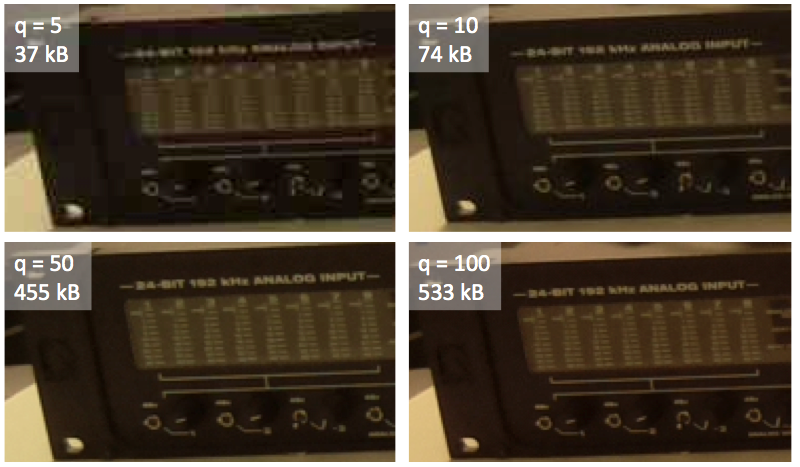
\includegraphics[width=.8\linewidth]{files/quality.png}
    \caption{Quality vs. image size considerations.}
    \label{fig:quality}
\end{figure}
The chosen quality value of 10\% is a trade-off between resolution and file size, the latter being limited by the capacity of the chosen router since the images are ultimately streamed on a server.
The image compression is implemented in such a way that the file size is not significantly reduced for quality values above approximately 20\% -- a quality of 50\% for example gives a file compression ratio of just 1.2 and a file size too large for the capacity of the router.
As shown in Figure~\ref{fig:quality}, however, the image resolution also does not decrease significantly for lower quality values, and the resolution for $q=10\%$ was sufficient for the current application. 
This quality value leads to a file size of $N_{pic} = \u{80}{kB}$ after the thumbnail -- a bitmap using unnecessary storage space -- is removed, corresponding to a compression ratio of 6.7.

As shown in \eqref{eq:required_capacity}, the file size generated leads to a required router capacity of approximately \u{3.12}{MB\per s}, given that, in the worst case, images from all 4 cameras are sent at once. 
A safety factor of 6 compared to the router's declared maximum capacity of $\u{150}{Mbps} = \u{18.75}{MB\per s}$ is thus obtained, which was required since, in practice, the router's maximum capacity was found to be much lower than the declared value.

\begin{equation}
  \label{eq:required_capacity}
  S_{required} = 4 \times \frac{\u{80/1024}{MB}}{\u{0.1}{s}} = \u{3.12}{MB\per s}
\end{equation}

The images are saved as \texttt{/tmp/stream/pic.jpg}, where \texttt{/tmp/stream/} is a folder with all permissions bits set, created for this purpose only. 
The current image is then taken from this folder by the \textit{mjpg-streamer} module which streams it on a webpage.
\footnote{The \textit{mjpg-streamer} is a Linux-UVC streaming application which steams JPGs from webcams, filesystems or other input plugins as \textit{M-JPEG} - a common video compression format - via HTTP to web browsers.}

\paragraph{Button}

A button is added to the Raspberry Pi such that it can be restarted or turned off without connecting to it. This allows the Raspberry Pi to be turned off correctly even when the network has not be set up properly or the ethernet is not working.
The button is a pull-down resistor, thus the signal at the output goes from 0 to 1 when the button is pressed. 
An interrupt is triggered when the button is pressed. 
It reads the button status once per second for six seconds and counts the number of times the button was in the ``down'' state. 
If, during this period, the ``down'' state is read at least 3 times, the system shuts down. Otherwise, the system reboots. 
The \texttt{python} script implementing this interrupt is shown in Code \ref{switchoff}.

\begin{center}
\begin{minipage}{0.9\linewidth}
    \begin{lstinputlisting}[caption=\texttt{$\sim$\/switchoff.py}, label=switchoff, language=Python, frame=none]{files/switchoff.py}
\end{lstinputlisting}
\end{minipage}
\end{center}


Both scripts above need to be executed on startup of the Raspberry. Therefore, the following lines are put in the file \texttt{/etc/rc.local}.
\begin{center}
\begin{minipage}{0.9\linewidth}
    \begin{lstlisting}[caption=\texttt{/etc/rc.local}, label=local, frame=none]
#Auto start camera
sudo /home/pi/start_camera.sh &
#Auto start shutdown
sudo python /home/pi/switchoff.py &
\end{lstlisting}
\end{minipage}
\end{center}

 \subsection{Audio Setup}
The tools used for the audio recording are two wireless audio transmitters with their corresponding receivers (\textit{Line 6 Relay G50}, see Figure \ref{fig:audio}) with the following key specifications:

  \begin{itemize}
      \item Frequency range 10 Hz - 20 kHz
      \item Distance range approx. 61 m (200 ft)
      \item Broadcast in 2.4 GHz band
  \end{itemize}

The transmitters are connected to microphones placed in the ears of the robot's acoustic head and the receivers are connected to two channels of a MOTU soundcard.
 
A conventional speaker is fixed on the robot as shown in Figure \ref{fig:speaker} and operated via the same soundcard. 
\subsection{Robot}

\begin{figure}
    \centering
    \begin{subfigure}{0.3\linewidth}
        \centering
        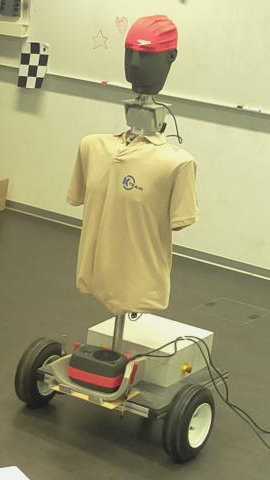
\includegraphics[height=0.3\textheight]{files/Robot2_cvt.png}
        \caption{Robot designed by Gigatec S.A. with acoustic head}
        \label{fig:robot}
    \end{subfigure}
    \hspace{0.5em}
    \begin{subfigure}{0.3\linewidth}
        \centering
        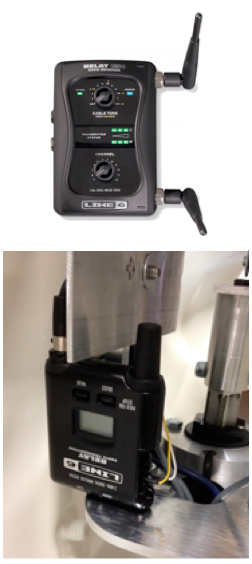
\includegraphics[height=0.3\textheight]{files/Wireless.png}
        \caption{Wireless audio receiver (top) and transmitter (bottom).}
        \label{fig:audio}
    \end{subfigure}
    \hspace{0.5em}
    \begin{subfigure}{0.3\linewidth}
        \centering
        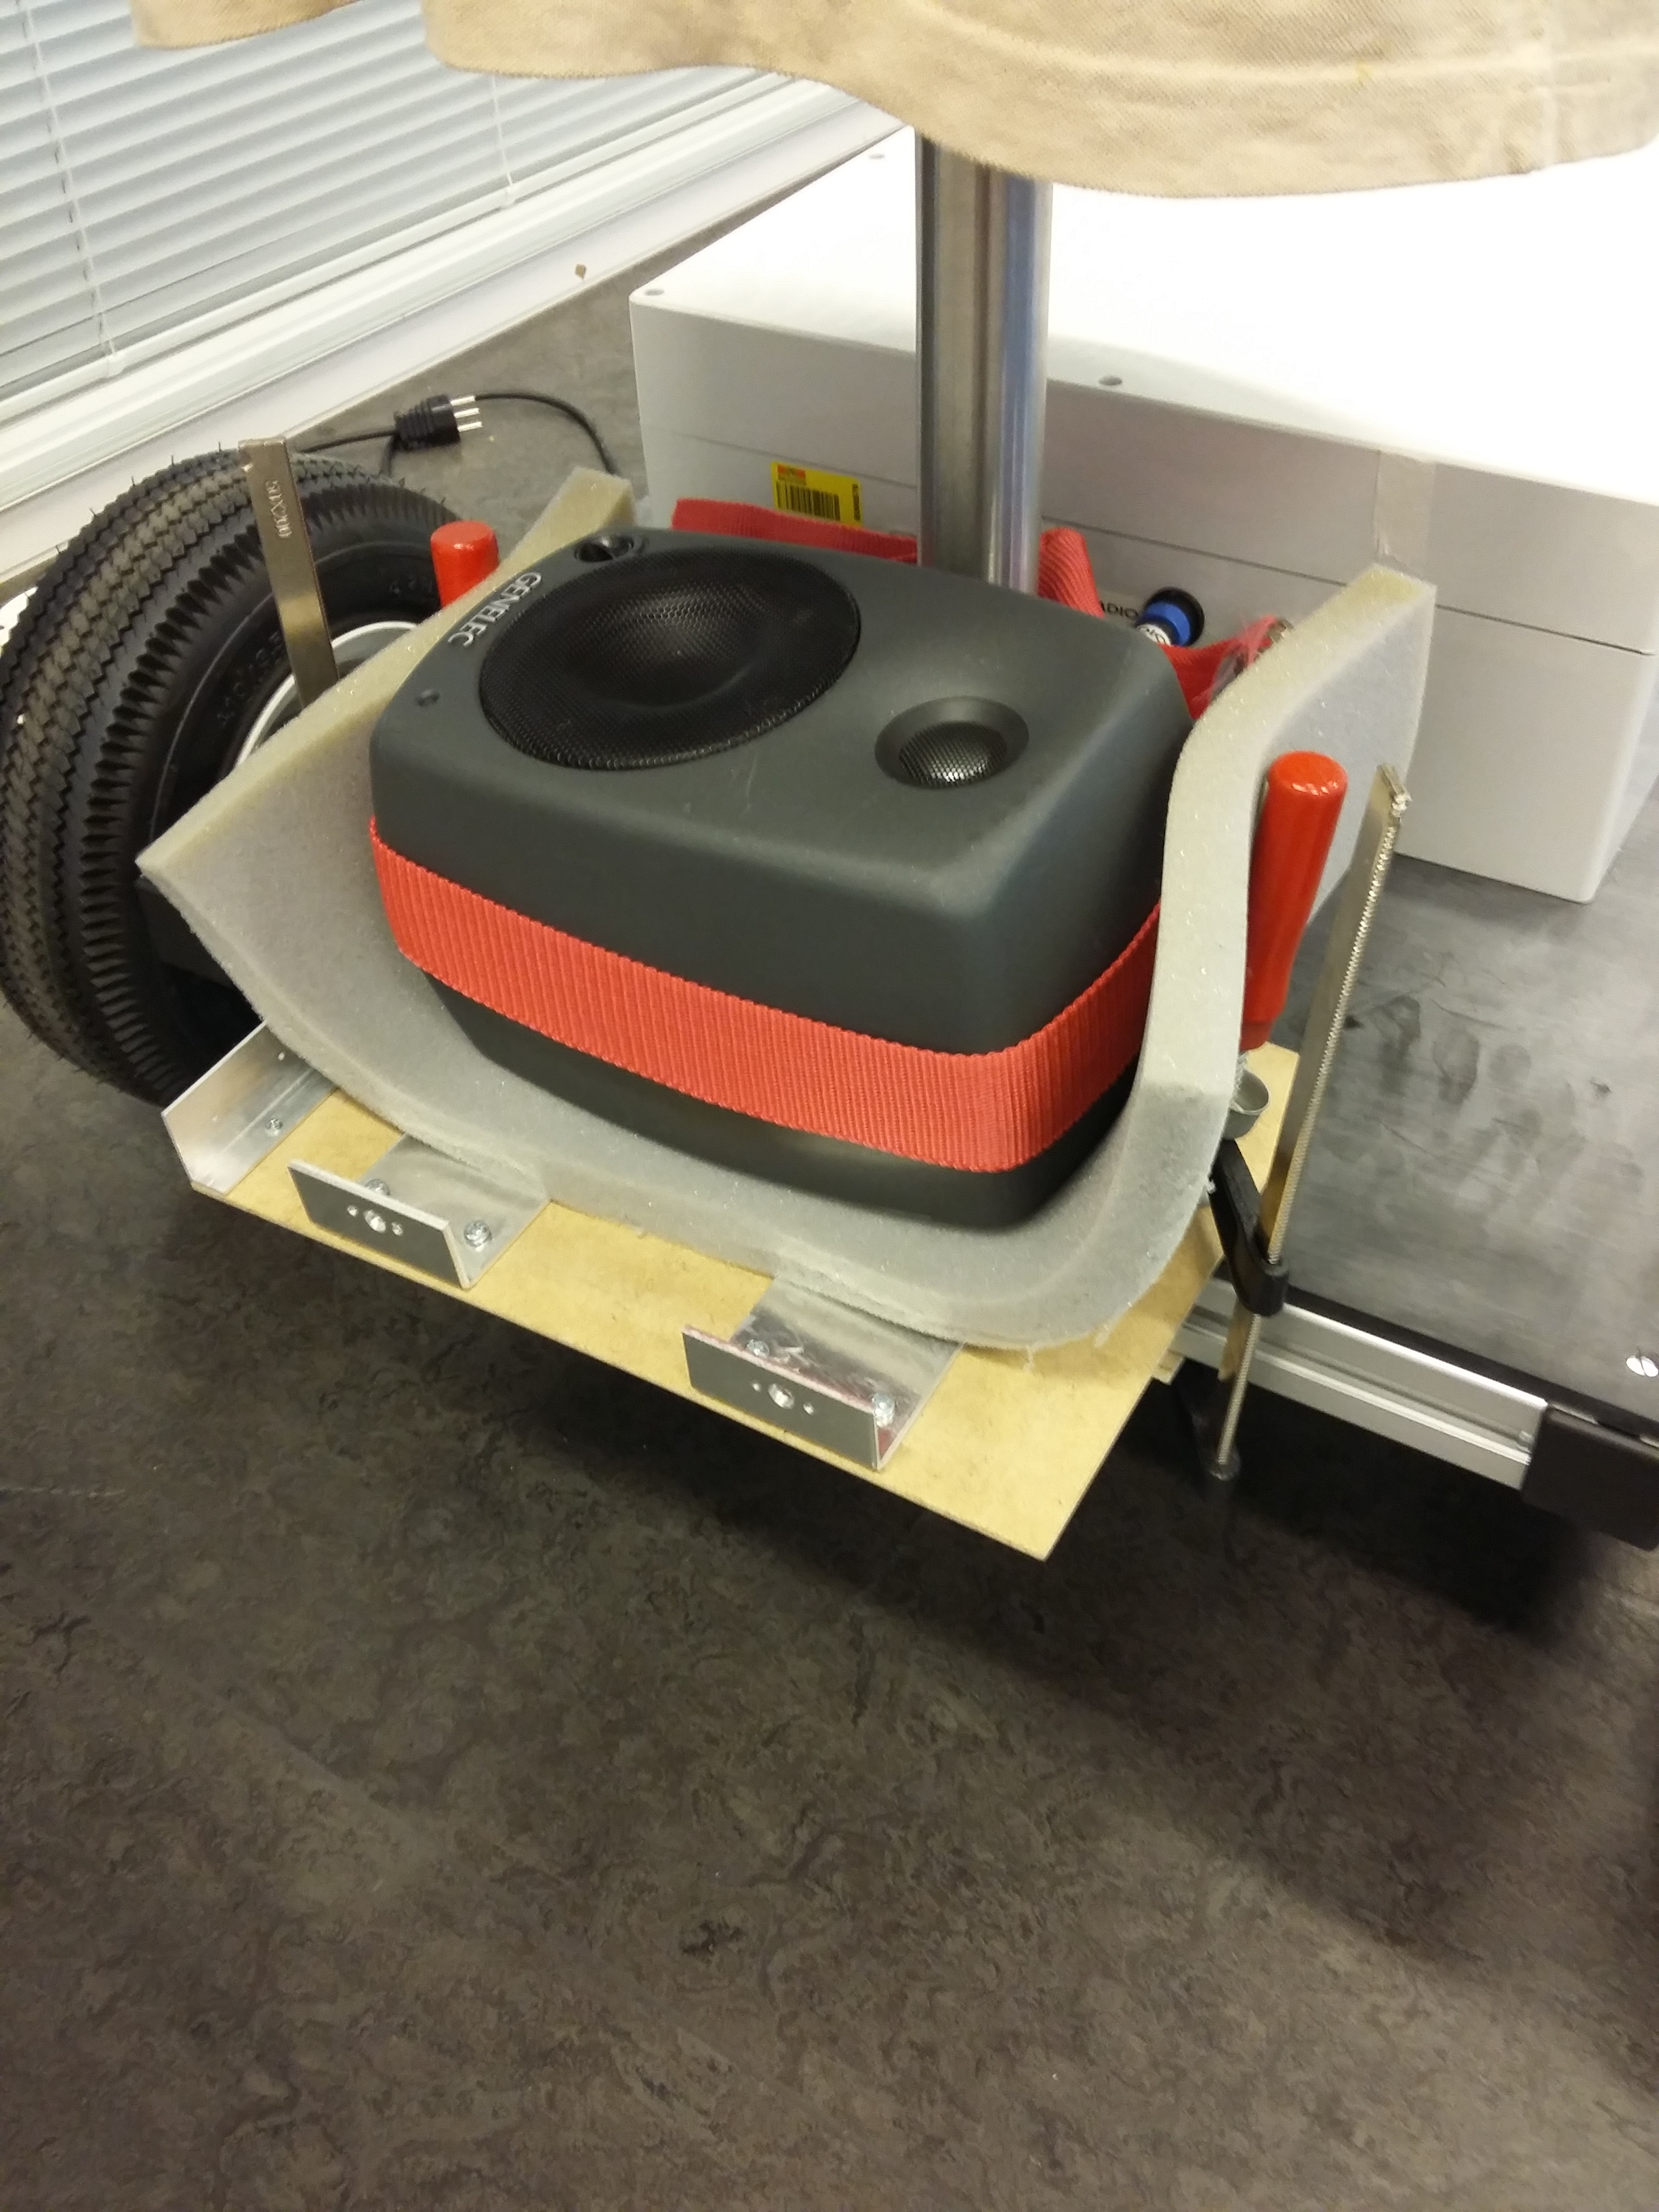
\includegraphics[height=0.3\textheight]{files/Speaker.jpg}
        \caption{Speaker fixation on the robot.}
        \label{fig:speaker}
    \end{subfigure}
    \caption{Robot designed by Gigatec S.A. for EchoSLAM with wireless audio equipment and speaker.}
\end{figure}

The robot used for the experiments was designed by Gigatec S.A. It is shown in Figures \ref{fig:robot}. 
Two wheels can be actuated for displacement (see § \ref{sec:movement}) and the acoustic head can be rolled, pitched and yawed independently. 
For the present setup, the head always stays in the standard (straight) position.

For autonomy, the robot is actuated via a socket interface and the AF\_INET protocol. All commands are sent via a \texttt{python} script. For manual operation of the robot, some commands can also be sent via ssh.
